\documentclass[11.5pt,sans,english]{article}
\usepackage[utf8]{inputenc}
\renewcommand{\familydefault}{\sfdefault}
 \usepackage[a4paper, total={7in, 9in}]{geometry}
\usepackage{listings}
\usepackage{color,colortbl}

\usepackage{fancyvrb}
\usepackage{xcolor}
\usepackage{tikz}
\usetikzlibrary{shapes,arrows}
\usepackage{multirow}
\usepackage{hyperref}
\usepackage{caption}
\usepackage{array}
\usepackage{tabularx}
\usepackage{wrapfig}

\usepackage{graphicx}
\graphicspath{{figs/}}

\hypersetup{
  pdfauthor={Lily Asquith},
  urlcolor=blue,
  colorlinks=true,
  linkcolor=purple,
  bookmarks=true
}

\definecolor{dkgreen}{rgb}{0,0.6,0}
\definecolor{gray}{rgb}{0.5,0.5,0.5}
\definecolor{mauve}{rgb}{0.58,0,0.82}

\lstset{frame=tb,
  language=python,
  aboveskip=3mm,
  belowskip=3mm,
  showstringspaces=false,
  columns=flexible,
  basicstyle={\small\ttfamily},
  numbers=none,
  numberstyle=\tiny\color{gray},
  keywordstyle=\color{blue},
  commentstyle=\color{dkgreen},
  stringstyle=\color{mauve},
  breaklines=true,
  breakatwhitespace=true,
  tabsize=3
}


\title{Y1 DT Guidance}
\author{Lily Asquith}
\date{Sept 2021}

\begin{document}

\tikzstyle{a} = [rectangle, draw, fill=green!20,  node distance=2.5cm,text width=5em, text centered, rounded corners, minimum height=2em]
\tikzstyle{line} = [draw, -latex']

\tikzstyle{restrictedcaf} = [draw, ellipse,fill=red!20, node distance=2.5cm,minimum height=2em]
    
    
    

%\maketitle
%
%\begin{abstract}
%This document details the containment studies for the NOvA FD.
%\end{abstract}
%
%
%\tableofcontents

%\newpage

\section{Timetable}

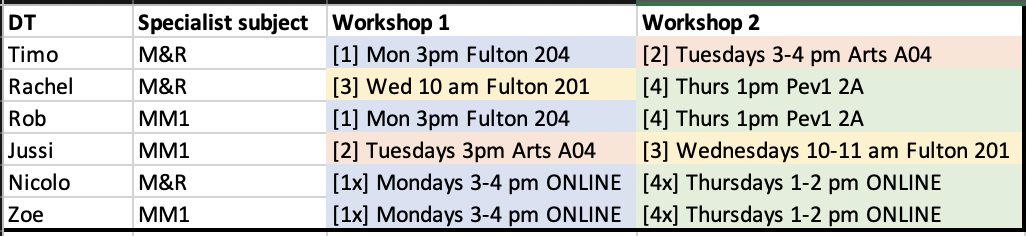
\includegraphics[scale=0.6]{DT-timetable}

\section{Face-to-face workshops}

\subsection{Preparation}
\begin{enumerate}
\item Ensure you have looked through the solutions for the workshop. Print a copy for yourself, but keep safe.
\item The MM1 problems and solutions are on: \href{ https://canvas.sussex.ac.uk/courses/20370/assignments}{the canvas page for MM1} under \texttt{Assignments/Weekly Problem Sets}.
\item The M\&R problems and solutions are on \href{https://github.com/dorksquith/TeachingFall2021/tree/main/DTs/Solvers}{Lily's github}.
\item If you notice any errors or if anything is unclear, let Lily or Alex know asap!
\end{enumerate}

\subsection{Arrival and setup}
\begin{enumerate}
\item Arrive at the allocated teaching space on the hour.
\item Login to the computer and have the workshop questions for both MM1 and M\&R ready to share on the projector.
\item Login to \href{https://www.polleverywhere.com}{Poll Everywhere }  username \texttt{ilovephysics} and the password given to you by Lily, navigate to the folder \texttt{2021/Workshops/}, and activate the poll "Workshop N questions".
\item Normally teaching sessions run from :00 to :50, but considering the current health and safety stuff for the pandemic, I would aim to start at 5 minutes past the hour and finish at 10 minutes to the hour.
\end{enumerate}

\subsection{Introduction}
\begin{enumerate}
\item Explain that the workshop should be roughly 20 mins each on MM1 and M\&R.
\item Ask the students to indicate any questions they are struggling with on the poll everywhere. They will almost certainly pick those that they are asked to submit the answers for for grading.
\item Tell the students that they should discuss and work together if they want to, and it is also fine to work alone if they wish.
\item Tell them that if they would like any answers checked or want anything clarified, to put their hand up.
\item Walk around the room to see if anyone needs a paper copy of the questions or has any questions.
\end{enumerate}


\subsection{Helping students}
\begin{enumerate}
\item If they show you an answer and it is numerically correct, let them know that it is. This is also fine to do for the highlighted questions for submission.
\item If they show you an answer and it is incorrect, read the question aloud with them and then go through their working step by step.
\item Remember that there is usually more than one way of solving a problem. Their method may not be wrong, but to save you having to determine this on the fly, a good technique is to say `right, this may well be a good method for solving this problem, but may I share with you the method I prefer?' - this way you can stick to the worked solutions we have provided you with.
\item If a student say they really don't understand, or really are struggling to make a start, check with them if they have attempted the adaptive practice assignments on canvas. Those assignments link the students to the sections of the eTextbook they should read. They may have had trouble getting on to canvas or setting up wiley - often I meet students who have almost no technical skills - if this is the case please get their email and email them and me so we can set up a time to get them going online. 
\end{enumerate}

\subsection{Finishing up}

Explain to the students that they should take a photo of their attempt at the highlighted questions and upload to the correct canvas page by the end of this week.

%Instructions for students:\\
%
%\includegraphics[scale=0.6]{student-instructions}

\section{Zoom workshops}

\textcolor{red}{Lily, Zoe, and Nicolo met on 30 Sept 2021 and concluded:} The best way to manage the \textbf{first week} of zoom workshops is to:\\[1ex]
1. Keep it simple! No polls or breakout rooms.\\
2. Keep it flexible! We will learn from the first week what does or does not work, and adjust accordingly.\\

Other than these two points, you should follow the instructions for in-person workshops.

\section{Marking}

Students will upload a photo of their answers to the workshop problems for MM1 and M\&R by Friday at noon (so the first for 2021 will be Friday 8th October).\\

The uploads will then be accessible via speedgrader from the respective canvas sites, filtered by student group (Axions etc).\\

The marking is out of 3:\\
\begin{itemize}
\item[0]: Nothing uploaded
\item[1]: Something uploaded, but nothing that makes sense. If they have uploaded a blank page for example, or if they have written the question but not attempted an answer. Or, if they uploaded just the answer, with no working.
\item[2]: An attempt has been made to solve the question, but it is not complete. For example (for the first M\&R question), they might have done the integral right but not solved the quadratic, or vice versa.
\item[3]. The correct answer is given.
\end{itemize}
\end{document}
